\documentclass[tikz, border=5mm]{standalone}
\usepackage[utf8]{inputenc}
\usepackage[european]{circuitikz}
\usepackage{amssymb} % <--- SOLUCIÓN: Paquete para poder usar \varnothing

\begin{document}
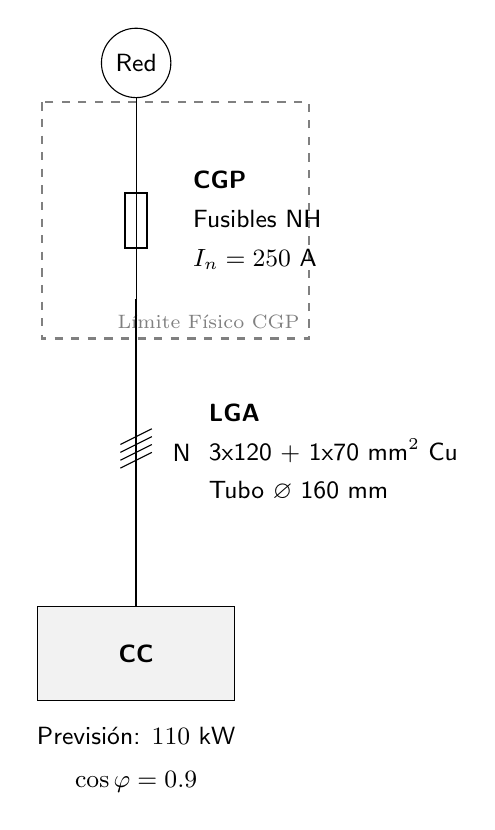
\begin{tikzpicture}[
    font=\small\sffamily
]

% ========================================================
% CUADRÍCULA DE AYUDA (Comenta o borra este bloque al final)
% ========================================================
% \draw[help lines, step=1cm, lightgray] (-3,-9) grid (3,1);
% \foreach \x in {-3,-2,-1,0,1,2,3} \node[anchor=north, font=\tiny, text=blue] at (\x,1) {\x};
% \foreach \y in {-9,-8,-7,-6,-5,-4,-3,-2,-1,0,1} \node[anchor=east, font=\tiny, text=blue] at (-3,\y) {\y};
% ========================================================


% 1. Origen: Red de Distribución
\node[draw, circle, minimum size=0.8cm, fill=white] (red) at (0,0) {Red};

% 2. CGP (Caja General de Protección)
% a) Dibujamos primero la envolvente física (la caja de poliéster) en línea discontinua
\draw[thick, dashed, gray] (-1.2, -0.5) rectangle (2.2, -3.5);
\node[text=gray, anchor=south east, font=\scriptsize] at (2.2, -3.5) {Límite Físico CGP};

% b) Dibujamos el interior (Acometida -> Fusible)
\draw (red) -- (0,-1) to[fuse] (0,-3) coordinate (cgp_out);
\node[right, align=left] at (0.6, -2) {\textbf{CGP}\\[3pt] Fusibles NH\\[3pt] $I_n = 250$ A};

% 3. Carga: CC (La dibujamos ANTES que la línea para que actúe de imán)
\node[draw, rectangle, minimum width=2.5cm, minimum height=1.2cm, fill=gray!10] (cc) at (0,-7.5) {\textbf{CC}};
\node[below=0.2cm] (prev) at (cc.south) {Previsión: $110$ kW};
\node[below=0.1cm] at (prev.south) {$\cos \varphi = 0.9$};

% 4. LGA (Conectamos directamente a cc.north, y guardamos el punto central)
\draw[thick] (cgp_out) -- (cc.north) coordinate[midway] (centro_lga);

% 5. Marcas unifilares paramétricas (se anclan al punto 'centro_lga')
\draw ([xshift=-0.2cm, yshift=0.1cm]centro_lga) -- ([xshift=0.2cm, yshift=0.3cm]centro_lga);
\draw ([xshift=-0.2cm, yshift=0.0cm]centro_lga) -- ([xshift=0.2cm, yshift=0.2cm]centro_lga);
\draw ([xshift=-0.2cm, yshift=-0.1cm]centro_lga) -- ([xshift=0.2cm, yshift=0.1cm]centro_lga);
\draw ([xshift=-0.2cm, yshift=-0.2cm]centro_lga) -- ([xshift=0.2cm, yshift=0.0cm]centro_lga) node[right=4pt] {N};

% Texto de la LGA
\node[right, align=left] at ([xshift=0.8cm]centro_lga) {\textbf{LGA}\\[3pt] 3x120 + 1x70 mm$^2$ Cu\\[3pt] Tubo $\varnothing$ 160 mm};

\end{tikzpicture}
\end{document}